\documentclass{article}
\usepackage[utf8]{inputenc}
\usepackage{graphicx}
\usepackage{epstopdf}
\usepackage{caption}
\usepackage{subcaption}
\usepackage{multirow}
\usepackage{hyperref}
\usepackage{url}
\usepackage{seqsplit}
\hypersetup{pdfstartview={FitH null null null}}
\usepackage{amssymb,amsmath}
\usepackage{amsthm}
\usepackage{empheq}
\usepackage{algorithm,algpseudocode}
\usepackage[margin=1.5in]{geometry}
\usepackage{listings}
\usepackage{program}
\lstset{language=Python} 

\usepackage{listings}
\usepackage{color} %red, green, blue, yellow, cyan, magenta, black, white
\definecolor{mygreen}{RGB}{28,172,0} % color values Red, Green, Blue
\definecolor{mylilas}{RGB}{170,55,241}


\title{Comparison of protein-protein docking prediction and optimization methods}
\author{Caiwei Wang, Xiaokai Qian, Sean Lander, \\Haipei Fan, Puneet Gaddam, Brett Koonce\\\\University of Missouri - Columbia}

\date{April 7, 2014}

\algloopdefx{NoEndIf}[1]{\textbf{If} #1 \textbf{then}}

\begin{document}

\maketitle

\section{Abstract}



\section{Introduction}



\section{Methods}



\subsection{Pipeline}

\begin{figure}[H]
\begin{center}
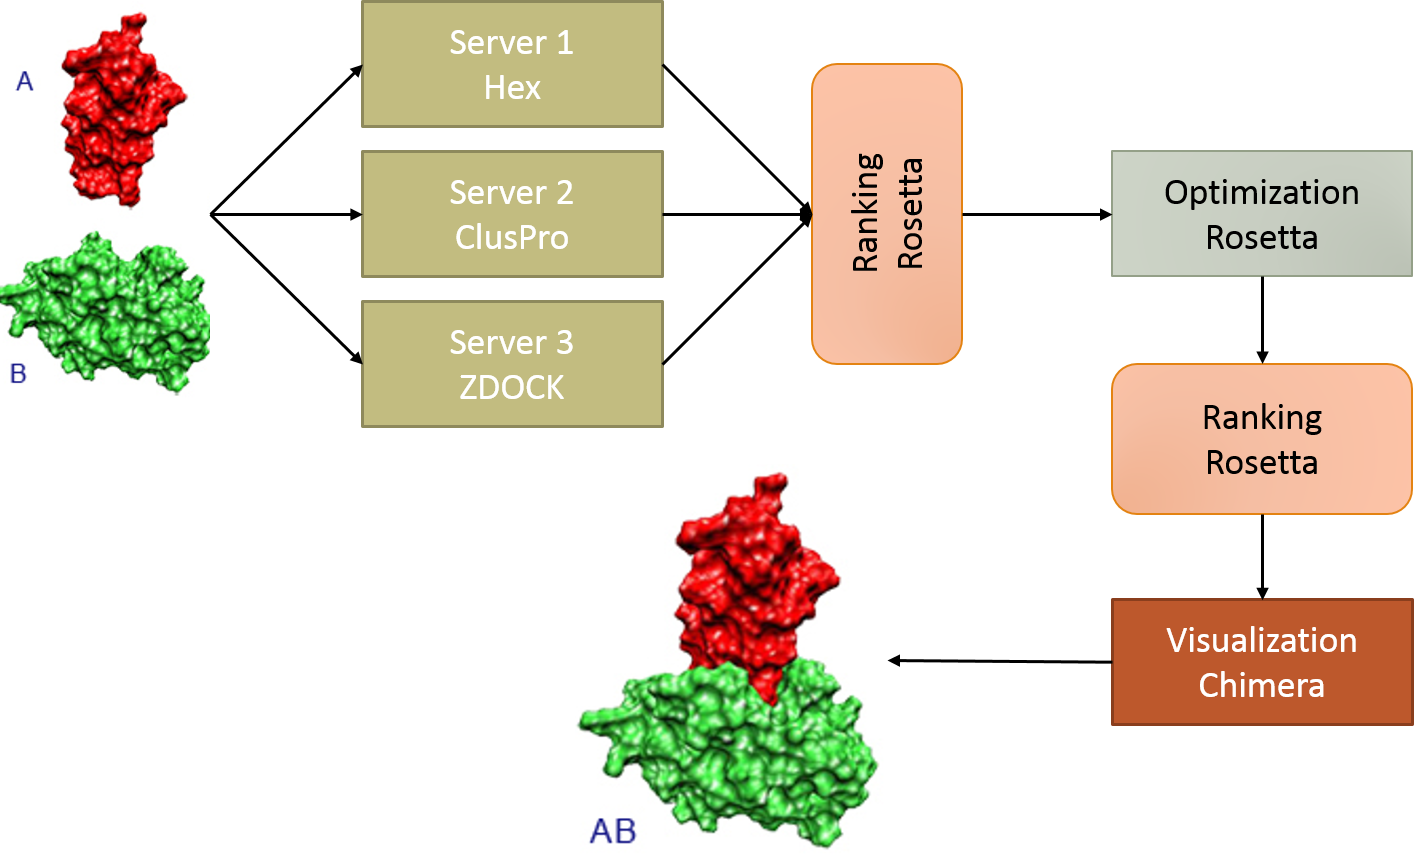
\includegraphics[width=\textwidth]{pipeline}
\caption{An overview of the comparison pipeline}
\label{Fig:blosum}
\end{center}
\end{figure}

\begin{enumerate}
\item Decoy Creation

\item Ranking

\item Optimization

\item Final Selection and Scoring
\end{enumerate}

\subsection{CAPRI Target Selection}

We selected the following template-free targets from the CAPRI database to build a model for: T53, T50.

\subsection{Pre-Processing}

\subsection{Decoy Creation}

\begin{enumerate}

\item Hex

\item ClusPro

\item ZDOCK

\end{enumerate}

\subsection{Decoy Optimization}

\begin{enumerate}

\item Decoy Ranking

\item Optimization

\end{enumerate}



\section{Results}

\subsection{Interface Creation}

\subsection{Scoring Methods - RMSD vs RosettaDock}

\begin{enumerate}

\item Before Optimization

\item After Optimization

\end{enumerate}

\subsection{Visualization}



\section{Conclusion}



\section{Citations}

We thank the following tools and papers: \\\\



\end{document}


\end{document}
